\documentclass[12pt]{article}
\usepackage{tikz}
\usepackage{verbatim}
\usepackage{listings}
   
\lstset{ %
%language=C++,                % the language of the code
basicstyle=\footnotesize,       % the size of the fonts that are used for the code
keywordstyle=\color{black}\bfseries,
%numbers=left,                   % where to put the line-numbers
%numberstyle=\footnotesize,      % the size of the fonts that are used for the line-numbers
%stepnumber=2,                   % the step between two line-numbers. If it's 1, each line 
%                                % will be numbered
%numbersep=5pt,                  % how far the line-numbers are from the code
backgroundcolor=\color{gray!20!white},  % choose the background color. You must add \usepackage{color}
%showspaces=false,               % show spaces adding particular underscores
showstringspaces=false,         % underline spaces within strings
showtabs=false,                 % show tabs within strings adding particular underscores
frame=single,                   % adds a frame around the code
%tabsize=2,                      % sets default tabsize to 2 spaces
%captionpos=b,                   % sets the caption-position to bottom
%breaklines=true,                % sets automatic line breaking
%breakatwhitespace=false,        % sets if automatic breaks should only happen at whitespace
title=\lstname,                 % show the filename of files included with \lstinputlisting;
% also try caption instead of title
%escapeinside={\%*}{*)},         % if you want to add a comment within your code
%morekeywords={*,...}            % if you want to add more keywords to the set
}

\usetikzlibrary{arrows}
\usetikzlibrary{shapes.multipart}
\usetikzlibrary{%
   decorations.fractals%
  ,decorations.pathmorphing%
  ,shadows%
}

\usepackage{hyperref}
\hypersetup{
bookmarks=false,         % show bookmarks bar?
unicode=true,          % non-Latin characters in Acrobat's bookmarks
pdftoolbar=true,        % show Acrobat's toolbar?
pdfmenubar=true,        % show Acrobat's menu?
pdffitwindow=true,     % window fit to page when opened
pdfstartview={FitH},    % fits the width of the page to the window
pdftitle={Swat guide},    % title
pdfauthor={Marcelo Zimbres Silva},     % author
pdfsubject={Spherical Wavelets},   % subject of the document
pdfcreator={Marcelo Zimbres Silva},   % creator of the document
pdfproducer={Marcelo Zimbres Silva}, % producer of the document
pdfkeywords={Wavelets} {Cosmic Rays}, % list of keywords
pdfnewwindow=true,      % links in new window
colorlinks=true,        % false: boxed links; true: colored links
linkcolor=red,          % color of internal links
citecolor=green,        % color of links to bibliography
filecolor=magenta,      % color of file links
urlcolor=cyan!50!black           % color of external links
}

% My definitions
%______________________________________________________________________

%\colorlet{swat}{yellow!50!black!50}
\colorlet{swat}{brown!50!black!50} % box color
\colorlet{textcolor}{brown!20!black} % text in box color
\colorlet{swatred}{red!50!black}

\tikzstyle{one}=[shade,top color=swat,fill=swat,rounded corners, textcolor,thick]
\tikzstyle{onel}=[rotate=-10,shade,top color=swat,fill=swat,rounded corners, textcolor,thick]
\tikzstyle{oner}=[rotate=10,shade,top color=swat,fill=swat,rounded corners, textcolor,thick]
\tikzstyle{inherit}=[open triangle 45-,thick,textcolor]
\tikzstyle{depend}=[draw,->,thick,textcolor,dashed]
\tikzstyle{code}=[draw,shade,rounded corners,text width=9cm]


\tikzstyle{two}=[anchor=north,shade,top color=swat,rectangle split, 
                     rectangle split parts=2, draw, text width=2.0cm,
		     fill=swat,rounded corners,textcolor,thick]

\tikzstyle{twonowidth}=[anchor=north,shade,top color=swat,rectangle split, 
                     rectangle split parts=2, draw, fill=swat,rounded corners,
		     textcolor,thick]


\tikzstyle{twored}=[anchor=north,shade,top color=swatred,rectangle split,
                        rectangle split parts=2,draw,text width=2.0cm,fill=swatred]

\tikzstyle{three}=[anchor=north,shade,top color=swat,rectangle split, rectangle split parts=3, draw, text width=3.0cm,fill=swat,
rounded corners,textcolor,thick]

\def\one{\node[style=one]}
\def\onel{\node[style=onel]}
\def\oner{\node[style=oner]}
\def\two{\node[style=two]}
\def\twonowidth{\node[style=twonowidth]}
\def\code{\node[style=code]}

\def\inherit{\draw[style=inherit]}
\def\depend{\draw[style=depend]}

\def\twored{\node[style=twored]}
\def\three{\node[style=three]}

%______________________________________________________________________
\begin{document}

  \parindent0pt
  \null
  \colorlet{mintgreen}{green!50!black!50}

  \thispagestyle{empty}
  \vskip3cm
  \vfill
  \hfil
  \begin{tikzpicture}[overlay]
    \coordinate (front) at (0,0);
    \coordinate (horizon) at (0,.28\paperheight);
    \coordinate (bottom) at (0,-.6\paperheight);
    \coordinate (sky) at (0,.62\paperheight);
    \coordinate (left) at (-.51\paperwidth,0);
    \coordinate (right) at (.51\paperwidth,0);

    \shade [bottom color=blue!30!black!10,top color=blue!30!black!50] ([yshift=-5mm]horizon -|  left) rectangle (sky -| right);

    %\shade [bottom color=black!70!green!25,top color=black!70!green!10] (front -| left) -- (horizon -| left)
    %   decorate [decoration=random steps] { -- (horizon -| right) } -- (front -| right) -- cycle;

    \shade [top color=black!70!green!25,bottom color=black!25] (front -| left) -- (horizon -| left)
      decorate [decoration=random steps] { -- (horizon -| right) } -- (front -| right) -- cycle;

    %\shade [top color=black!70!green!25,bottom color=black!25] ([yshift=-0mm]front -| left) rectangle ([yshift=1pt]front -| right);

    \fill [black!25] (bottom -| left) rectangle ([yshift=3mm]front -| right);

    \def\nodeshadowed[#1]#2;{\node[scale=2,above,#1]{#2};\node[scale=2,
        above,#1,yscale=-1,scope fading=south,opacity=0.4]{#2};}

    \node[at={(-0,6  )}] {\Huge \textsc{\bf \textcolor{red!50!black!90}{SWAT}}}; 
    \node[at={(-0,4  )}] {\Huge {\bf\color{gray!70!black} The \textcolor{red!50!black!90}{S}pherical \textcolor{red!50!black!90}{W}avelet \textcolor{red!50!black!90}{A}nalysis \textcolor{red!50!black!90}{T}ool}};

    \one (TObject) at (-8,15) {\Large \bf\color{gray!70!black} TObject};
    \one (TArrayD) at (-3,15) {\Large \bf\color{gray!70!black}TArrayD};
    \one (TDKernel) at (2,15) {\Large \bf\color{gray!70!black}TDKernel};
    \one (TCoeffInfo) at (7,15) {\Large \bf\color{gray!70!black}TCoeffInfo};

    \one (TNamed) at (-8,13) {\Large \bf\color{gray!70!black}TNamed};
    \one (TVMap) at (-3,13) {\Large \bf\color{gray!70!black}TVMap};
    \one (TEulerAngle) at (2,13) {\Large \bf\color{gray!70!black}TEulerAngle};
    \one (TAngDistance) at (7,13) {\Large \bf\color{gray!70!black}TAngDistance};

    \one (TSkyMap) at (-8,11) {\Large \bf\color{gray!70!black}TSkyMap};
    \one (TWignerd) at (-3,11) {\Large\bf\color{gray!70!black} TWignerd};
    \one (TWavMap) at (2,11) {\Large \bf\color{gray!70!black}TWavMap};
    \one (TAlm) at (7,11) {\Large \bf\color{gray!70!black}TAlm};

    \one (TSphHarmB) at (-8,9) {\Large \bf\color{gray!70!black}TSphHarmB};
    \one (TSwatB) at (-3,9) {\Large \bf\color{gray!70!black}TSwatB};
    \one (TSwatF) at (2,9) {\Large \bf\color{gray!70!black}TSwatF};
    \one (TSphHarmF) at (7,9) {\Large \bf\color{gray!70!black}TSphHarmF};
   
   %_______________________________________________________
   \draw[draw,-open triangle 45,thick,color=gray] (node cs:name=TNamed) -- (node cs:name=TObject);
   \draw[open triangle 45-,thick,gray] (node cs:name=TDKernel,anchor=south) |- +(0,-1)  node (y) {};
   \draw[open triangle 45-,thick,gray] (node cs:name=TCoeffInfo,anchor=south) |- +(0,-1)-- +(-10.0,-1);
   \draw[open triangle 45-,thick,gray] (node cs:name=TArrayD,anchor=south) -- (node cs:name=TVMap);
   \draw[draw,-open triangle 45,thick,gray] (node cs:name=TVMap) -- (node cs:name=TNamed);
   \draw[draw,-open triangle 45,thick,gray] (node cs:name=TSkyMap) -- (node cs:name=TVMap);
   \draw[draw,-open triangle 45,thick,gray] (node cs:name=TWavMap) -- (node cs:name=TVMap);
   \draw[draw,->,thick,gray,dashed] (node cs:name=TWavMap) -- (node cs:name=TSwatB) node[midway,sloped,above]           {};
   \draw[draw,->,thick,gray,dashed] (node cs:name=TWavMap) -- (node cs:name=TAlm) node[midway,sloped,above]             {};
   \draw[draw,->,thick,gray,dashed] (node cs:name=TSkyMap) -- (node cs:name=TSphHarmB) node[midway,sloped,above]        {};
   \draw[draw,->,thick,gray,dashed] (node cs:name=TSwatB) -- (node cs:name=TWignerd) node[midway,sloped,above]          {};
   \draw[draw,->,thick,gray,dashed] (node cs:name=TSphHarmB) -- (node cs:name=TWignerd) node[midway,sloped,above]       {};
   \draw[draw,->,thick,gray,dashed] (node cs:name=TWavMap) -- (node cs:name=TEulerAngle) node[midway,sloped,above]      {};
   \draw[draw,->,thick,gray,dashed] (node cs:name=TAngDistance) -- (node cs:name=TEulerAngle) node[midway,sloped,above] {};
   \draw[draw,->,thick,gray,dashed] (node cs:name=TAlm) -- (node cs:name=TSwatF) node[midway,sloped,above]              {};
   \draw[draw,->,thick,gray,dashed] (node cs:name=TAlm) -- (node cs:name=TSphHarmF) node[midway,sloped,above]           {};

   %_______________________________________________________

   \node[at={(0,-3.0)}] {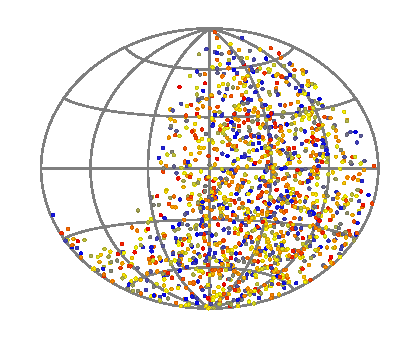
\includegraphics[scale=2.0]{skymap.pdf}};

   \node[at={(0,-10)}] {\Large\bf \color{gray!70!black}Manual for version 1.44 - Marcelo Zimbres};
   %\draw[-,very thick,gray] (-9,-10.5) -- (9,-10.5);

  \end{tikzpicture}
  \vfill


\newpage
\tableofcontents

\newpage
\section{Introduction} \label{ch::Introduction}

\href{http://www.ifi.unicamp.br/~mzimbres}{SWAT} is a package for analysis of
functions that live on the sphere, which I have mostly used to analyze data 
collected by the Pierre Auger experiment and CRPropa simulations. I have written it from
scratch as part of my my Ph.D. It evolved from a simple ROOT macro and
got bigger and bigger, since the code may be useful to other people I decided
to organize, document it and make it public. The code is an C++ implementation
of the spherical wavelet transform as presented in \cite{wiaux}. Some
attractive features of SWAT are:

\begin{list}{\labelitemi}{}
\item Harmonic and Wavelet transform on the sphere.
\item Interface to Healpix code, which is included in the build system.
\item Easy selection of events hitting sky window. 
\item Calculation of deflection vs. $1/E$ graphs.
\item ROOT and FFTW are the only prerequisites.
\end{list}

The package includes some parts of the Healpix code. There are two reasons why
I decided to include it here, instead of just link against Healpix libraries.
\begin{enumerate}
\item I do not need all Healpix routines and support to the fits format. 
\item I usually need shared libraries to call Healpix code in a ROOT session,
which are not built by Healpix build system since most of its code are C++
templates.
\end{enumerate}

Most of the theoretical details of analysis of functions defined on $S^2$ and $S^3$ 
were taken from \cite{wiaux} and references therein. 

The code has been tested in \textsc{Linux} and \textsc{MacBook}, but the code
is portable enough to be built on other platforms.  In the following we
describe how to use SWAT. Questions concerning the software can sent to Marcelo
Zimbres \href{mailto:mzimbres@gmail.com}{mzimbres@gmail.com}
\vspace{0.7cm}
\newline
{\bf \large Acknowledgements}
\vspace{0.7cm}

Most of SWAT were developed with financial support from CAPES.  Additionaly I
would like to acknowledge the Institute of Physics at UNICAMP and the Bergische
Universit\"at Wuppertal for finacial support, Brunel University for granting me a
scholarship to participate in the Cern School of Computing, the Ettore Majorana
Foundation and Center for scientific Culture, the brasilian group of the Pierre
Auger experiment, with special thanks to my supervisor Ernesto Kemp, for
beliving in the project and Rafael Alves Batista for testing the code. The
Pierre Auger Group at university of Wuppertal, with special thanks to Nils
Niertenh\"ofer for helping me with CRPropa.

\subsection{Installation} \label{ch::installation}
As a prerequisite to install SWAT you need ROOT and FFTW installed, the
configure script will fail if they are not installed. SWAT uses autotools to
generate the configure script and the Makefile, so you can expect all the
standard configure options and makefile targets. The lines bellow will install
the libraries on {\color{brown}"/usr/local"}
{\bf \color{brown}
   \begin{lstlisting}
   $ ./configure CXXFLAGS="-O3 -ffast-math"
   $ make
   $ make install
   \end{lstlisting}
}
The flags passed to the configure script are optional, but greatly improve performance.
To use some of the features of the package, I am assuming you are able to build
shared libraries on your platform. To easy the task of loading swat libraries
the macro load.C, will be installed on
{\color{brown}"prefix/share/swat"}. To load the libraries in ROOT's C++
interpreter you just have to execute it in your ROOT session, or just add it to
your code {\color{brown}.rootlogon.C} macro.

{\bf \color{brown}
\begin{lstlisting}
$ cp /usr/local/shar/swat/load.C ~/.rootlogon.C
$ root # The .so's are automatically loaded here.
\end{lstlisting}
}

All SWAT classes are now available in the ROOT session with syntax
highlighting. You should also be able to generate documentation in HTML format
with the macro {\color{brown}"prefix/share/swat/makehtml.C"}. You have to run
this macro from the directory where you built SWAT. The documentation will be
built in the directory {\color{brown}htmldoc}.

\subsection{Getting ready} \label{ch::ready}
To use Herald data, you will have to convert the ascii file to a {TTree} and
save it in a .root file, for that you should use the macro
{\color{brown}prefix/share/swat/convert\_herald.C} where prefix is usually
{\color{brown}/usr/local}.  Copy this macro to the same directory where you have the
herald data file. The macro will read a file with name
{\color{brown}"herald.dat"}, so you may have to rename your file or edit the macro. 
For CRPropa simulations you can just configure CRPropa to output a .root file
instead of a text file.  The code uses the title of the TTree to differentiate
between a Herald and CRPropa file. The title of the TTree for CRPropa must be
\textit{\color{brown}"CRPropa 3D events"}, as far as I know, this is the default.

\subsection{High quality graphs with pgfplots} \label{ch::pgfplots}
If you have pgfplots installed on your machine, you can use the \LaTeX\,\,
files which are available in the directory pgfplots to generate high quality
graphs using some output of swat analysis. You may have noted that after
running {\color{brown}swatfind} you get many text files in your working
directory. They are input files for the \LaTeX\,\, files. In the following
subsections we show how to use the material.
\subsubsection{Skymaps}
When you run the program swatfind or swatsim, they produce a file named
skymap.dat. This file contains the coordinates and energy of the events that
passed the cut. To generate a graph for an isotropic sky for example, one can
use:
{\bf \color{brown}
\begin{lstlisting}
$ tar -xzf skymap.tar.gz
$ cd skymap
$ swatsim -n 1000 -s 1
$ pdflatex --jobname=skymap-f1 skymap.tex
\end{lstlisting}
}
Example skies can be seem here:\\
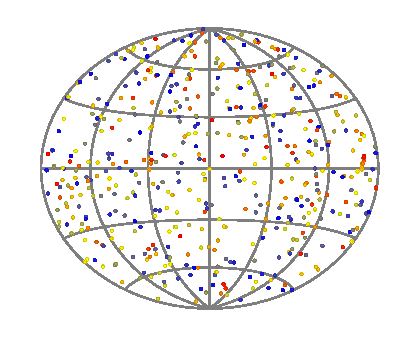
\includegraphics[scale=1.0]{skymap-sim.pdf} 
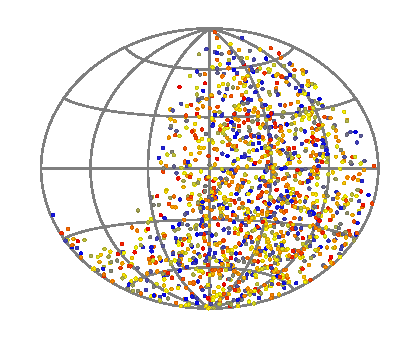
\includegraphics[scale=1.0]{skymap.pdf}
The program will also generate the file mult\_cand.tex, this file contains only
the events which hit the tangent plane in the position found by the wavelet
analysis. An example can be seem below on the left side. On the right side we
see a skymap simulated with CRPropa. \\
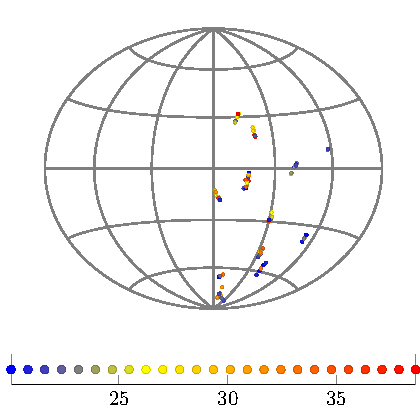
\includegraphics[scale=1.0]{mult-cand.pdf} 
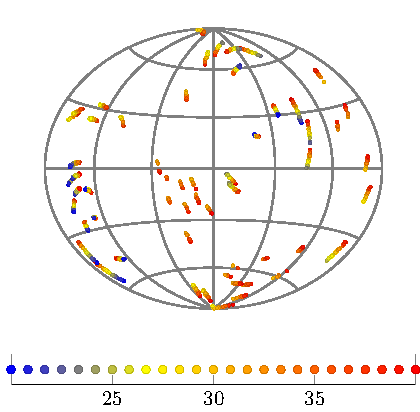
\includegraphics[scale=1.0]{crpropa.pdf}

Usually the energy of events is represented in skymaps as circles of varying
size, where events with higher energy have larger circles. I do not like such
representations since they can give the false impression that the angular
resolution gets worse as the energy increases, which is not true. Additionally,
these circles pollute the figure. In the representations I am using, colors
are used to differentiate energies which in my opinion is a much clear way of
representing the sky.

\subsubsection{Energy deflection graphs}
In addition to skymap.dat, the files {\color{brown}corr\_graphN.dat} will be also generated, 
with N varying from 0 to 15. These files contains the energy-deflection graphs,
of the events the hit the tangent plane in the position found by the wavelet
analysis. On the figure below, we see two examples. The graph on the left
originates from a CRPropa simulation. \\
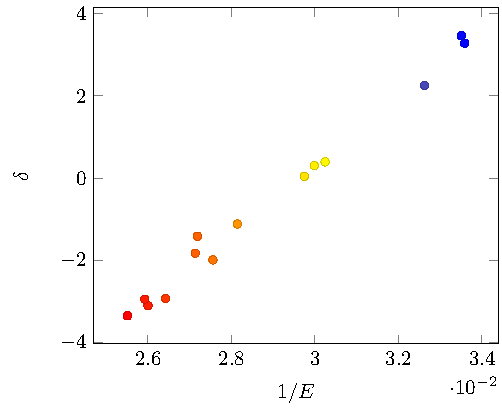
\includegraphics[scale=0.8]{corr_graph.pdf} 
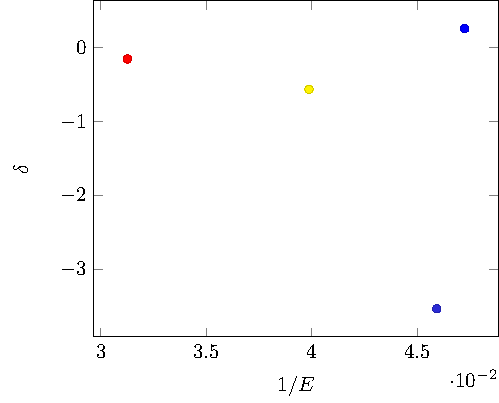
\includegraphics[scale=0.8]{corr_graph-sim.pdf} \hfill

\subsubsection{Number of events versus orientation}

The number of events hitting stripes centered at the same point and
whose orientation varies from 0 - 180 degrees is also a useful observable
when interpreting the results. Some of these graphs can be seem below:

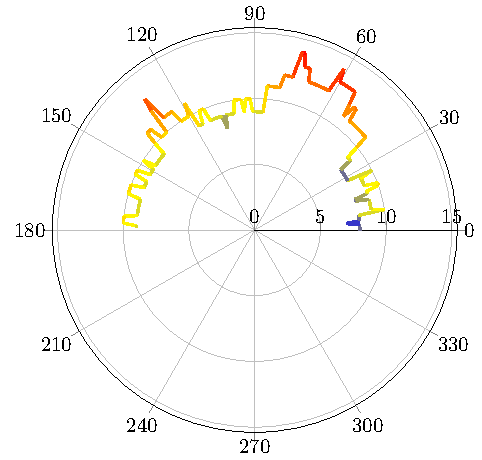
\includegraphics[scale=0.8]{multiplicity.pdf}  
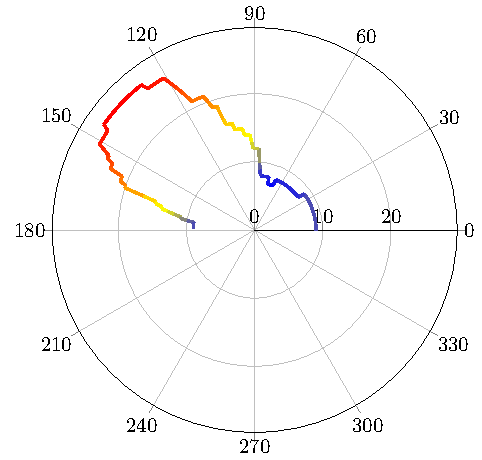
\includegraphics[scale=0.8]{multiplicity-sim.pdf} 

To generate them, use the macro {\color{brown}multiplicity.tex} in the pgfplots directory
and the file {\color{brown}multiplicity0.dat} generated by swatfind of swatsim.
One such file will be generated for each source found.
Similar to what we have done for the energy deflection graphs.


\subsubsection{Wigner-d functions}

Swat implements the calculation of the wigner-d functions via FFT.
You can use the file pgfplots/wignerd.tar.gz to generate some nice graphs.


\includegraphics[scale=1.0]{wignerpolar.pdf}
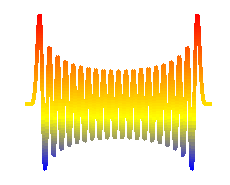
\includegraphics[scale=1.0]{wigner.pdf} 
\section{Transforms on the Sphere}
Most SWAT functionality is based on Fourier and wavelet transforms on the sphere, therefore we give
in this section a brief overview of analysis of functions on the sphere. Before
that however, it is important to mention the problem of sampling functions on
the sphere, which is refered to as its pixelization.  Due to the fact
that most of the time we work with function defined on the line (temporal
series, for example) or on the plane (images in general) we do not have to care
much about how to sample. We simply divide it in squares of same area and everything works
just fine. However, when we try the same thing on the sphere we imediately see
that it is impossible to achieve same area pixelization on the sphere due its curvature.

There are two main features we would like to have decide to divide a Sphere in
bins. First we would like to have bins of same area, this is achieved by the
Healpix pixelization \ref{healpix}. Second, we would like to to use FFT to calculate
functions on the sphere instead of slow recursion and that is achieved by ECP
Pixalization, which stands for "Equidistant cylindrical projection"\ref{healpix}.
Unfortunately theses two features are mutualy excludente. In this software we
decided to use ECP due to its simplicity. In ECP, the three Euler angles, which we 
are using to parametrize SO(3), are sampled as follows
$\alpha$, $\beta$ and $\gamma$
\begin{equation}
\alpha_{j_1} = \gamma_{j_1} = \frac{2\pi j}{2B}, \ \ \ \beta_{j_1} = \frac{\pi(2k + 1)}{4B}
\nonumber
\end{equation}
\begin{figure}[ht]
   \centering
      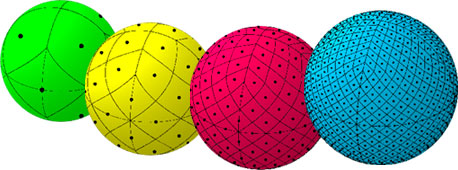
\includegraphics[height=4cm,width=10.78cm,angle=0]{healpixGridRefinement.jpg} \\
      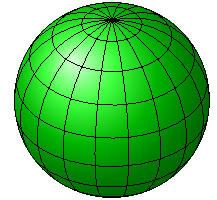
\includegraphics[]{cylindrical-f1.pdf}
      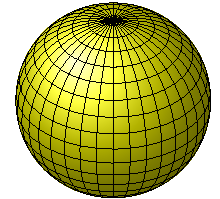
\includegraphics[]{cylindrical-f2.pdf}
      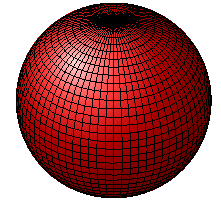
\includegraphics[]{cylindrical-f3.pdf}
   \caption{Above:Healpix pixelization of the sphere. Below: The ECP pixelization.}
   \label{healpix}
\end{figure}

\subsection{Fourier Transform on SO(3)}
A function $f \in L^2(SO(3))$ can be decomposed as follows
\begin{eqnarray}
f(\alpha,\beta,\gamma) = \sum_{l = 0}\sum_{m = -l}^l\sum_{n = -l}^l f^l_{mn}D^l_{mn}(\alpha,\beta,\gamma).
\label{back}
\end{eqnarray}
where
\begin{eqnarray}
D^l_{mn}(\alpha,\beta,\gamma) = e^{-im\alpha}d^l_{mn}(\beta)e^{-in\gamma}.
\end{eqnarray}
is called "Wigner-D functions" and form an irreducible representation on SO(3). The
functions $d^l_{mn}$ are called "small wigner-d functions".

The inverse of \ref{back} on ECP pixelization is given by
\begin{equation}
f^l_{mn} = \frac{1}{(2B)^2}\sum_{j_1 = 0}^{2B - 1}\sum_{j_2 = 0}^{2B - 1}\sum_{k = 0}^{2B - 1}
w_B(k)f(\alpha_{j_1},\beta_{k},\gamma_{j_1})D^{l*}_{mn}(\alpha_{j_1},\beta_{k},\gamma_{j_1})
\end{equation}
where $B$ is the band limit and the quadrature weights are given by
\begin{equation}
w_B(k) = \frac{2}{B}\sin\left(\frac{\pi(2k + 1)}{4B}\right)\sum_{j = 0}^{B - 1}
\frac{1}{2k + 1}\sin\left((2j+1)(2k+1)\frac{\pi}{4B}\right)
\end{equation}
where $0\le k < 2B$. 

\section{The three main programs}
In the following sub-sections we will describe the three main programs which 
SWAT installs and which provide an easy interface to the wavelet analysis.
\subsection{swatfind}
{\it swatfind} is the main program. It can be used to find sources in Pierre
Auger data and CRPropa simulations. Beyond that, it can be also used to test
whether the events belong to a multiplet, calculating energy-deflections graphs
for the sources found. All information is saved in .root format. A source here
is a term used to mean something with a position on the sky, usually described
by $(\theta,\phi)$ and an orientation. We will use the three Euler angle
$(\alpha,\beta,\gamma)$ to describe the source. 

It uses the following algorithm:
\begin{enumerate}
\item The TTree containing Pierre Auger data or CRPropa simulations
is read from the file passed in the command line with option -f.
\item Events with energy in the range $emin < E < emax$ are selected and used
to fill a Healpix map.  The options -i and -e are used to pass the energy range.
\item The Healpix map generated is transformed to wavelet space. The parameter
$N$, passed by the option -N gives the precision on the ability of the wavelet
to find the angle $\gamma$, which can range from 1 - 128 in our implementation. 
The precision in degrees are calculated with the formula $180/N$ The scale on
which the analysis is performed is passed with option -j. It ranges from 0 - 8.
We found out that the best results are achieved with j = 1.
\item A partial sort is used to find the 15 largest wavelet coefficients.
\item The euler angles found will be used to calculated the tangent plane
equation for each source. The width and length of the plane are passed with
options -w and -l respectively.
\item A loop on the data is made to select all events hitting the tangent
plane. The energy cut is used again.
\item The energy-deflection graphs are calculated and the correlations found
are printed on the screen.
\end{enumerate}
All the information is saved in the file {\color{brown}"sources.root"}.  Lets see an example:

{\bf \color{brown}
\begin{lstlisting}
$ swatfind -j 1 -N 127 -i 20 -e 40 -w 2 -l 10 -f chain.root
TFile**		chain.root	CRPropa output data file
 TFile*		chain.root	CRPropa output data file
  OBJ: TNtuple	events	CRPropa 3D events
  OBJ: TEventList	list	20 < emin && emax < 40 
  OBJ: THealpixMap	hmap	Healpix sky map
  OBJ: TGraph	g0	C = -0.993, N = 4 
  OBJ: TGraph	g1	C = -0.986, N = 5
  OBJ: TGraph	g2	C = 0.000, N = 0
  OBJ: TGraph	g3	C = -1.000, N = 2
  ...
\end{lstlisting}
}

The N in the TGraph title is the number of events in the graph (or the number of 
events which hit the tangent plane) and is not to be confused with the N passed by command line
option -N. C is the correlation of the energy-deflection graphs.

Now, if you want to see the exact location of the source:
{\bf \color{brown}
\begin{lstlisting}
$ root sources.root
root[1] .ls
TFile**		sources.root	
 TFile*		sources.root	
  KEY: THealpixMap	hmap;1	Healpix sky map
  KEY: TEulerAngle	source0;1	
  KEY: TEulerAngle	source1;1	
  KEY: TEulerAngle	source2;1	
root [2] source0->Show(1)
wav(137.812,-27.4219,159.638) = -0.035312
root [3] 
\end{lstlisting}
}
\subsection{swatsim}
{\it swatsim} uses Monte Carlo simulations to calculate the probability of a multiplet happen by 
chance on a isotropic sky. We still do not have means of simulating exposure, a feature which should be 
added in future versions. The probability is calculated as follows: 
\begin{itemize}
\item The program simulates n isotropic skies. If you want to add your simulated events
to each sky you can use the option -f and a TTree in CRPropa format will be read
and added in each sky.
\item For each sky simulated the analysis made by swatfind is used to calculate the
correlation coefficient. The tangent plane is calculated for the largest wavelet coefficient found.
\item If the correlation is larger than C , passed with option -c and has more than n events, passed 
with option -m, then the multiplet has passed the criteria.
\item The probability will be total number of multiplets passing the criteria divided by 
number of skies simulated.
\end{itemize}

Beyond the probability, the program outputs two additional histograms:
\begin{enumerate}
\item A histogram of the correlation coefficients found, for which the total number
of events is larger than the value passed with -m.
\item A histogram of the number of events in the tangent plane.
\end{enumerate}

\subsection{swat}
swat: This program is only used to benchmark and test the algorithm. It can test
both the spherical harmonic transform and the spherical wavelet transform.
{\bf \color{brown}
\begin{lstlisting}
$ time swat -J 8 # Will test spherical harmonic transform.
$ time swat -J 8 -N 3 # Will test wavelet transform.
\end{lstlisting}
}

\appendix
\section{swatfind}
{\bf \color{brown}
   \begin{lstlisting}
 Calculates sources from herald data, additionaly
 calculates correlation of events hitting tangent plane
 and dispalys on the screen. The results are saved to
 sources.root file. To convert a Herald file to the
 format used by this progra use the macro
 macros/convert_herald.C in swat source tree.
 
 Usage: prog [ -j scale] [-N number] [-i emin] [-e
 emax] [-w width] [-l length] [-f file.root]

 Options:

 -h: This menu.
 -j: Wavelet scale a number in the range 0 <= j <= 8,
     defaults to 1.
 -N: Band limit of wavelet, in the range 0 < N <= 128,
     defaults to 1.
 -i: Minimum energy of events, defaults to 20 EeV.
 -e: Maximum energy of events, defaults to 40 EeV.
 -w: Width of tangent plane, defaults to 2 degrees.
 -l: Length of tangent plane, defaults to 10 degrees.
 -f: Root file containing Tree with data, defaults to
     chain.root.
   \end{lstlisting}
}
\newpage
\section{swatsim}
{\bf \color{brown}
   \begin{lstlisting}
 Calculates the probability of a multiplet with minimum
 correlation C (see -c option) and minimum number of
 events m (see -m option) happen by chance, using
 wavelet analysis.  First an isotropic sky is simulated
 and the wavelet representation of the sky is
 calculated, the euler angles of the largest
 coefficient is used to calculate the equations of the
 tangent plane at the position found (the euler
 angles). The correlation C is calculated including all
 events that hit the tangent plane, whose size is
 specified with the options -l and -w. The probablility
 will be the number of multiplets with correlation > C
 and number of events > m, diveded by the number of
 skies simulated.  Additionaly, two other quantities
 are calculated, the histogram of the number of events
 that hit the tangent plane and the histogram of the
 C's found for which the number of events is greater
 than m (passed in the command line). If -f option is
 used, TTree in the file will be read and events will
 be added to the analysis, this is useful to include a
 simulated multiplet on the analysis, hiding it in the
 isotropic backgroung the test the algorithm.

 Usage: swatsim [ -j scale] [-N number] [-n nevents]
 [-s skies] [-i emin] [-e emax] [-c corr] [-m mevents]
 [-w width] [-l length] [-f file.root]

    Options:

  -h: This menu.
  -j: Wavelet scale a number in the range 0 <= j <= 8,
      defaults to 1.
  -N: Band limit of wavelet, in the range 0 < N <= 128,
      defaults to 1.
  -n: Number of events in the simulated sky,
      defaults to n = 1000
  -s: Number of skies to simulate, defaults to 100.
  -i: Minimum energy of events, defaults to 20 EeV.
  -e: Maximum energy of events, defaults to 40 EeV.
  -c: Minimum correlation, defaults to 0.2.
  -m: Minimum number of events hitting tangent plane.
  -w: Width of tangent plane, defaults to 2 degrees.
  -l: Length of tangent plane, defaults to 10 degrees.
  -f: Add events in TTree stored in file to the
      simulated sky.
   \end{lstlisting}
}

\section{swat}
{\bf \color{brown}
   \begin{lstlisting}
    Tests the algorithm doing a forward an backward
    transform.

    Usage: swat [-J scales] [-N band-limit]

    Options:

    -h: This menu.
    -J: TAlm object in root file. If not provided, the
        program will compare input and output for J = 7 and
        return true if diffrence less that 10e-10.  
    -N: Band limit of wavelet to be used.
   \end{lstlisting}
}

\begin{thebibliography}{99}
\bibitem{frm} J Fourier Anal Appl (2008) 14: 145–179.
\bibitem{wiaux} Mon. Not. R. Astron. Soc. 000, 1–22 (2007). 
\bibitem{swat} \url{http://www.ifi.unicamp.br/~mzimbres/}
\end{thebibliography}
\end{document}

